
%----------------------------------------------------------------------------------------
%	PACKAGES AND THEMES
%----------------------------------------------------------------------------------------

\documentclass{beamer}

\mode<presentation> {

% The Beamer class comes with a number of default slide themes
% which change the colors and layouts of slides. Below this is a list
% of all the themes, uncomment each in turn to see what they look like.

%\usetheme{default}
%\usetheme{AnnArbor}
%\usetheme{Antibes}
%\usetheme{Bergen}
%\usetheme{Berkeley}
%\usetheme{Berlin}
%\usetheme{Boadilla}
%\usetheme{CambridgeUS}
%\usetheme{Copenhagen}
%\usetheme{Darmstadt}
%\usetheme{Dresden}
%\usetheme{Frankfurt}
%\usetheme{Goettingen}
%\usetheme{Hannover}
%\usetheme{Ilmenau}
%\usetheme{JuanLesPins}
%\usetheme{Luebeck}
\usetheme{Madrid}
%\usetheme{Malmoe}
%\usetheme{Marburg}
%\usetheme{Montpellier}
%\usetheme{PaloAlto}
%\usetheme{Pittsburgh}
%\usetheme{Rochester}
%\usetheme{Singapore}
%\usetheme{Szeged}
%\usetheme{Warsaw}

% As well as themes, the Beamer class has a number of color themes
% for any slide theme. Uncomment each of these in turn to see how it
% changes the colors of your current slide theme.

%\usecolortheme{albatross}
%\usecolortheme{beaver}
%\usecolortheme{beetle}
%\usecolortheme{crane}
%\usecolortheme{dolphin}
%\usecolortheme{dove}
%\usecolortheme{fly}
%\usecolortheme{lily}
%\usecolortheme{orchid}
%\usecolortheme{rose}
%\usecolortheme{seagull}
%\usecolortheme{seahorse}
%\usecolortheme{whale}
%\usecolortheme{wolverine}

%\setbeamertemplate{footline} % To remove the footer line in all slides uncomment this line
%\setbeamertemplate{footline}[page number] % To replace the footer line in all slides with a simple slide count uncomment this line

\setbeamertemplate{navigation symbols}{} % To remove the navigation symbols from the bottom of all slides uncomment this line

\definecolor{water}{HTML}{3fb0ac}
\colorlet{beamer@blendedblue}{water}

\usebackgroundtemplate%
{
		
		 %  
\includegraphics[scale=0.5]{res/logo.png} 
		      
}

\setbeamertemplate{footline}
{
\vspace{1.5cm}
  \leavevmode%
  \hbox{%
    \begin{beamercolorbox}[wd=.9\paperwidth,ht=2.25ex,dp=1ex,center]{title in head/foot}%
      \usebeamerfont{title in head/foot}\pgfsetfillopacity{1}\insertshorttitle
    \end{beamercolorbox}%
    \begin{beamercolorbox}[wd=.1\paperwidth,ht=2.25ex,dp=1ex,right]{date in head/foot}%
      \insertframenumber{} / \inserttotalframenumber\hspace*{2ex}
    \end{beamercolorbox}}%
  \vskip0pt%
}



}

\usepackage{graphicx} % Allows including images
\usepackage{booktabs} % Allows the use of \toprule, \midrule and \bottomrule in tables
\usepackage[german]{babel}
\usepackage[utf8x]{inputenc}
\usepackage{textpos}
\usepackage{multimedia}
%----------------------------------------------------------------------------------------
%	TITLE PAGE
%----------------------------------------------------------------------------------------

\title[Autorisierungsmanagement für eine virtuelle
Forschungsumgebung für Geodaten: Abschlusspräsentation]{Autorisierungsmanagement für eine virtuelle
Forschungsumgebung für Geodaten \\ \textbf{ABSCHLUSSPRÄSENTATION}} % The short title appears at the bottom of every slide, the full title is only on the title page

\author[]{
Bachvarov, Aleksandar\\
Dimitrov, Atanas\\
Mortazavi Moshkenan, Houraalsadat\\
Sakly, Khalil\\
Slobodyanik, Anastasia\\
Voneva, Sonya\\ \vspace{.75cm}
	
\includegraphics[width=6.5cm, height=1.5cm]{res/logos} 
} 

\date{19. März 2018} % Date, can be changed to a custom date

\begin{document}

\begin{frame}[plain]
\titlepage % Print the title page as the first slide
\end{frame}


%----------------------------------------------------------------------------------------
%	PRESENTATION SLIDES
%----------------------------------------------------------------------------------------
\addtobeamertemplate{frametitle}{}{%
\begin{textblock*}{70mm}(.90\textwidth,-1cm)

\includegraphics[height=1cm,width=1cm]{res/logo}
\end{textblock*}}


\begin{frame}
\frametitle{Einleitung}
\framesubtitle{Ziel des Produkts}

\begin{itemize}
	\item<1-7> Zugriffsanfragen senden
	\item<2-7> Ressource nutzen
	\item<3-7> Ressource erstellen
\end{itemize}
	\begin{figure}
		
			\includegraphics<4-7>[height=2cm,width=2cm]{res/benutzer}
			\hspace{0.2cm}
			\includegraphics<5-7>[height=2cm,width=2cm]{res/ressbesitzer}
			\hspace{0.2cm}
			\includegraphics<6-7>[height=2cm,width=2cm]{res/admin}	
			\item<7>Benutzer, Ressourcenbesitzer und Administrator
			
	\end{figure}

\end{frame}
%------------------------------------------------
\begin{frame}

\frametitle{Architektur}
\framesubtitle{Model-View-Template}
\vspace{1cm}
\includegraphics[width=\textwidth]{res/mvt}

\end{frame}
%------------------------------------------------
\begin{frame}
\frametitle{App-Funktionalität 1/3}
\begin{center}
\movie[height = \textheight, width = \textwidth, autostart]{}{res/User.avi}

\end{center}\end{frame}
%------------------------------------------------
\begin{frame}
\frametitle{App-Funktionalität 2/3}
\begin{center}
\movie[height = \textheight, width = \textwidth, autostart]{}{res/Owner.avi}

\end{center}\end{frame}
%------------------------------------------------
\begin{frame}
\frametitle{App-Funktionalität 3/3}
\begin{center}
\movie[height = \textheight, width = \textwidth, autostart]{}{res/Admin.avi}

\end{center}\end{frame}
%------------------------------------------------
\begin{frame}

\frametitle{Wie haben wir das gemacht}
\framesubtitle{Statistik}
\begin{figure}
	
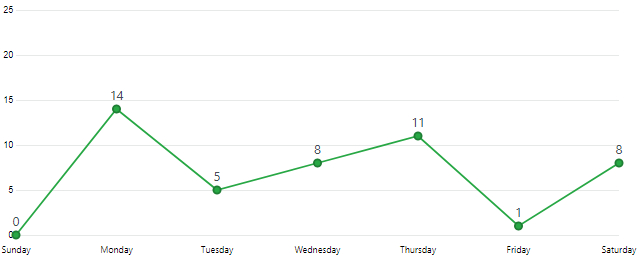
\includegraphics[width=.8\textwidth, height = 4cm]{res/git_stat}\newline \vspace{0.3cm}
\#Commits für die Woche 22-28.01.2018
\includegraphics[width=\textwidth]{res/stat}
\end{figure}

\end{frame}
%------------------------------------------------
\begin{frame}
\frametitle{Wie haben wir das gemacht}
\framesubtitle{Tools}
\includegraphics<1>[width=6.7cm, height=3.2cm]{res/tools1}
\includegraphics<2>[width=\textwidth]{res/tools2}
\includegraphics<3>[width=\textwidth]{res/tools3}
\includegraphics<4>[width=\textwidth]{res/tools4}
\end{frame}
%------------------------------------------------
\begin{frame}
\frametitle{Arbeitsprozess}
\framesubtitle{Was hat gut funktioniert}
\begin{itemize}
	\item<1-3> Zeitplanung
	\item<2-3> Aufgabenverteilung
	\item<3> Einarbeitung in Django
\end{itemize}
\end{frame}
%------------------------------------------------

\begin{frame}
\frametitle{Arbeitsprozess}
\framesubtitle{Was war aufwändiger als gedacht}
\begin{itemize}
	\item<1-3> Planungsphase
	\item<2-3> Wasserfallmodell ohne Rückkopplung
	\item<3> Entwurf vs. Implementierung
\end{itemize}
\end{frame}

%------------------------------------------------
\begin{frame}
\frametitle{Schlussfolgerung}
	
\begin{figure}
\includegraphics[width=0.65\textwidth]{res/trio}
\end{figure}
\end{frame}

%----------------------------------------------------------------------------------------

\end{document}